\documentclass[paper=letter, fontsize=12pt]{article}

\usepackage[english]{babel} % English language/hyphenation
\usepackage{amsmath,amsfonts,amsthm} % Math packages
\usepackage[section]{placeins}  % prevent figures / eqns / tables 
                                % from slipping out of section.
\usepackage{sectsty} % Allows customizing section commands
\allsectionsfont{\centering \normalfont\scshape} % Make all sections centered, 
                                                 % the default font and small 
                                                 % caps 

\usepackage{fancyhdr} % Custom headers and footers

% algorithms
\usepackage{algorithm}
\usepackage[compatible]{algpseudocode}

\usepackage{ragged2e} % Text alignment
\usepackage[margin=1in]{geometry} % 1 inch margins
\usepackage{tikz} % Not always necessary, but allows very customizable 
                  % figures / object placement
\usepackage{enumitem} % get more out of enumerate

% begin additional packages
\usepackage{hyperref}
\usepackage{blindtext}
\usepackage[
    backend=biber,
    url=false, 
    doi=true,
    eprint=true
]{biblatex}
\addbibresource{./references.bib}
% end additional packages

% Header and Footers
\pagestyle{fancyplain} % Makes all pages in the document conform to the custom 
                       % headers and footers
\fancyhead{} % No page header
\fancyfoot[L]{} % Empty left footer
\fancyfoot[C]{} % Empty center footer
\fancyfoot[R]{\thepage} % Page numbering for right footer
\renewcommand{\headrulewidth}{0pt} % Remove header underlines
\renewcommand{\footrulewidth}{0pt} % Remove footer underlines
\setlength{\headheight}{13.6pt} % Customize the height of the header

% Number all figs, eqns, and tables within the section
\numberwithin{equation}{section} % Number equations within sections 
\numberwithin{figure}{section} % Number figures within sections 
\numberwithin{table}{section} % Number tables within sections 

\setlength\parindent{4pt} % 4pt indentation for paragraphs
\setlength{\parskip}{\baselineskip} % adds some spacing in between paragraphs

\newcommand{\horrule}[1]{\rule{\linewidth}{#1}} % Create horizontal rule command
                                                % with 1 argument of height
\newcommand{\fancyline}{\\ \horrule{0.5pt} \vspace{0.1cm}} % fancy line to put
                                                           % under questions

%  Some commands for algorithm environments                                            
\renewcommand{\algorithmicrequire}{\textbf{Input:}}
\renewcommand{\algorithmicensure}{\textbf{Output:}}
\renewcommand{\algorithmicforall}{\textbf{for each}}
\newcommand{\algorithmiccontinue}{\textbf{continue}}
\algloopdefx{RETURN}[1][]{\textbf{return} #1}

% useful math shortcuts
\newcommand{\lagr}[1]{\mathcal{L}\left( #1 \right)}
\newcommand{\expval}[1]{E\left[#1\right]}
\newcommand{\var}[1]{\text{var}\left(#1\right)}
\renewcommand{\det}[1]{\text{det}\left(#1\right)}
\newcommand{\diag}[1]{\text{diag}\left[#1\right]}

% begin additional definitions and commands

% end additional definitions and commands

%-------------------------------------------------------------------------------
%	TITLE SECTION
%-------------------------------------------------------------------------------

\title{	
\normalfont \normalsize 
\textsc{RICE UNIVERSITY COMP540} \\ [25pt]
\horrule{0.5pt} \\[0.4cm] % Thin top horizontal rule
\huge deton8: Detector of Nuclei \\ % The assignment title
\horrule{2pt} \\[0.5cm] % Thick bottom horizontal rule
}

\author{Will LeVine \& Gabriel Vacaliuc}

\date{\normalsize\today}

\begin{document}

\maketitle

\begin{abstract}
    \blindtext
\end{abstract}

\newpage

\tableofcontents

\newpage


%-------------------------------------------------------------------------------
%   CONTENT
%-------------------------------------------------------------------------------

\section{Introduction}

Modern medical research generates an incredible amount of data that requires
significant time to be processed in some way.  Often some of this processing
involves tedious manual hand labeling of data, such as images, simulations, or
video.  To this end, it is desirable for medical research to develop automated
processes so as to allow trained professionals to focus on more challenging
problems than rote labeling.  An example of one of these problem ripe to be
solved is the labeling of microscopic cell nuclei in image data.  As such, the
2018 Data Science Bowl is focused on solving this problem, or at least
advancing the current state of the art.  We've included the corresponding
\href{https://www.kaggle.com/c/data-science-bowl-2018}{kaggle competition}'s
description below:

\begin{quote}
    \textbf{\large Spot Nuclei. Speed Cures.}

    Imagine speeding up research for almost every disease, from lung cancer and
    heart disease to rare disorders. The 2018 Data Science Bowl offers our most
    ambitious mission yet: create an algorithm to automate nucleus detection.

    We've all seen people suffer from diseases like cancer, heart disease,
    chronic obstructive pulmonary disease, Alzheimer's, and diabetes. Many have
    seen their loved ones pass away. Think how many lives would be transformed
    if cures came faster.

    By automating nucleus detection, you could help unlock cures faster—from
    rare disorders to the common cold. Want a snapshot about the 2018 Data
    Science Bowl? \href{https://www.youtube.com/watch?v=eHwkfhmJexs}{View this
    video.}

    \textbf{\large Why nuclei?}

    Identifying the cells' nuclei is the starting point for most analyses
    because most of the human body's 30 trillion cells contain a nucleus full
    of DNA, the genetic code that programs each cell. Identifying nuclei allows
    researchers to identify each individual cell in a sample, and by measuring
    how cells react to various treatments, the researcher can understand the
    underlying biological processes at work.

    By participating, teams will work to automate the process of identifying
    nuclei, which will allow for more efficient drug testing, shortening the 10
    years it takes for each new drug to come to market.
    \href{https://datasciencebowl.com/2018dsbtutorial/}{Check out this video
    overview to find out more.}
\end{quote}

To begin understanding the task at hand, we're going to dive in and check out 
some images from the dataset.  We'll continue by explaining exactly what needs
to be done for a given image, followed by some commentary on the specific 
challenges of this competition.

\subsection{Dataset Examples}

The dataset contains an assortment of images of sizes ranging from (256, 256)
to (1024, 1024), however most images are on the smaller end.  Upon reading in
our images, we reshape them all to (256, 256) for simplicity.  Observe a sample
of our dataset in Figure \ref{fig:dsbowl18-grid}.

\begin{figure}
    \centering
    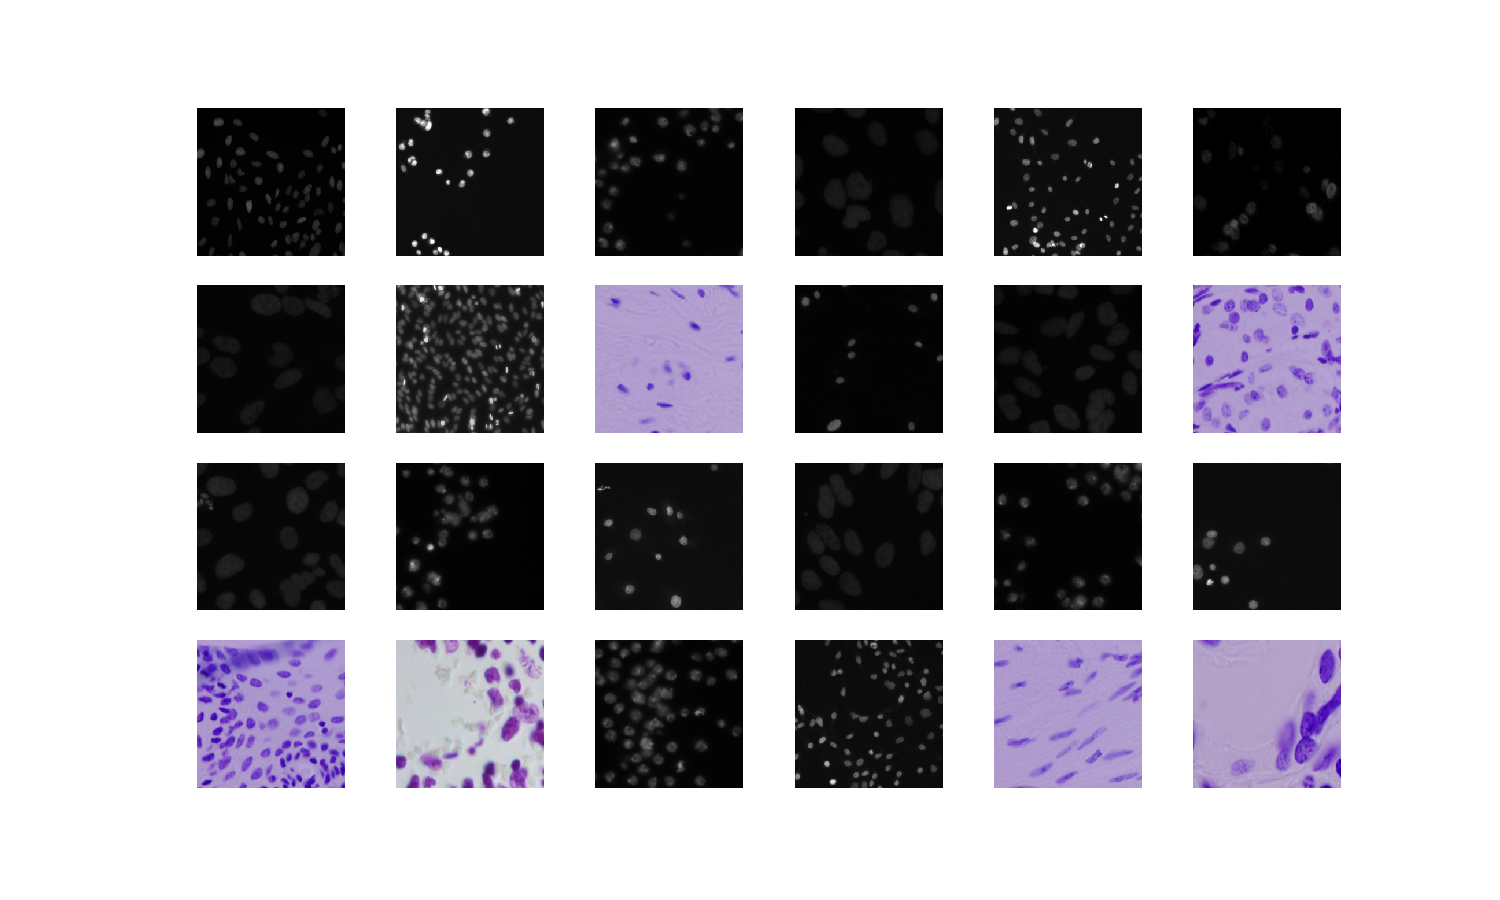
\includegraphics[width=\textwidth]{./figs/dsbowl18-imagegrid-4x6.png}
    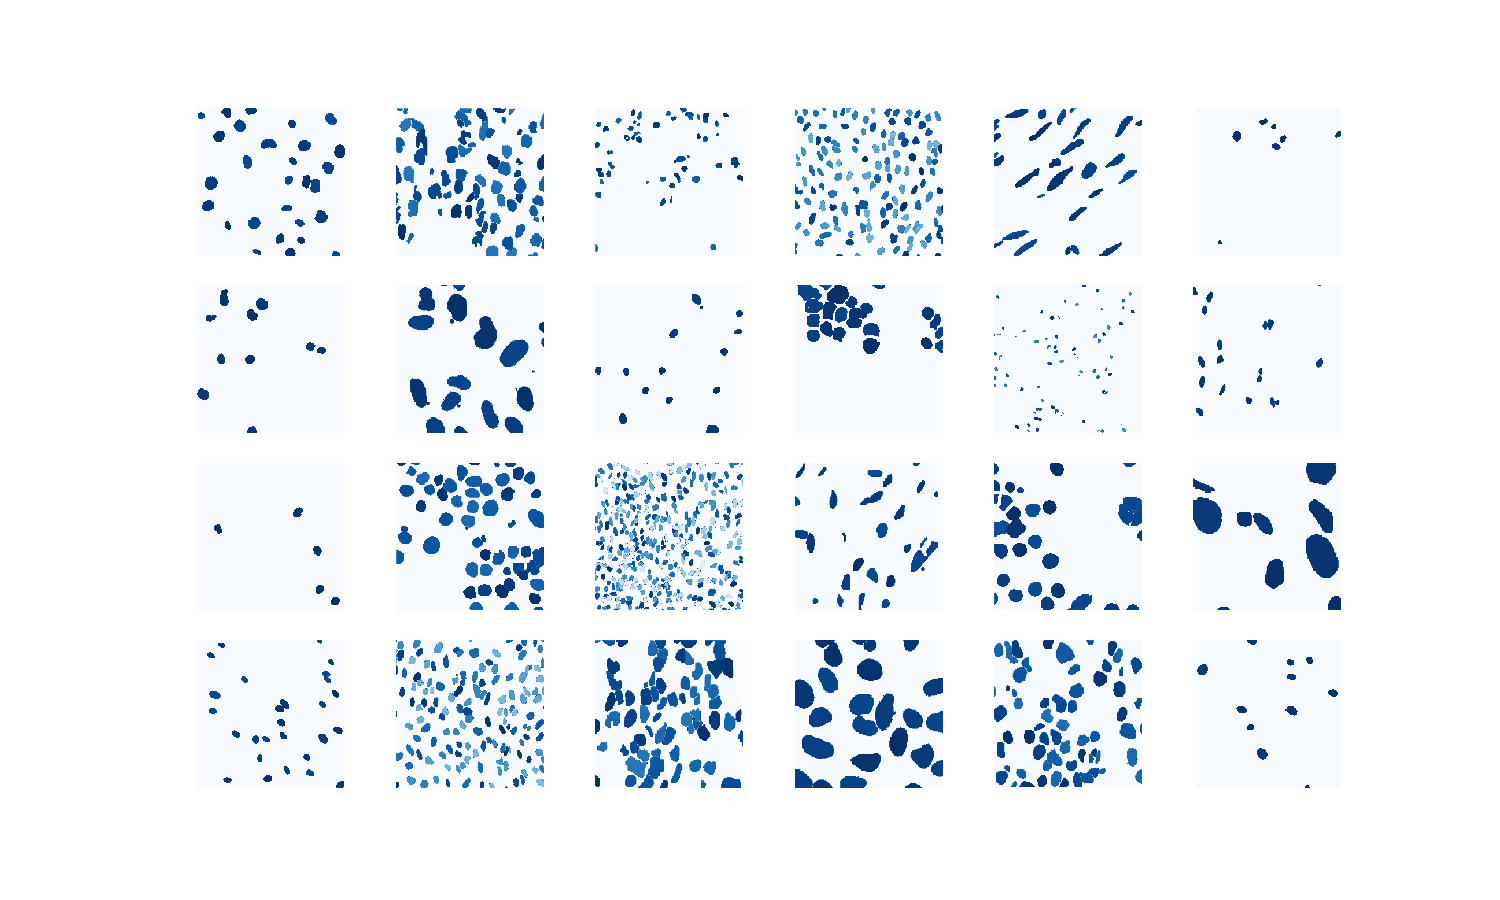
\includegraphics[width=\textwidth]{./figs/dsbowl18-imagegrid-masks-4x6.png}
    \caption{An assortment of images from our dataset.  All have been resized
    to 256 x 256. (top) raw image data (bottom) true masks }
    \label{fig:dsbowl18-grid}
\end{figure}

\subsection{Formal Description of Task}

Here is a mathematical description of our task.  Given a dataset $\mathcal{D}$
composed of images, $x \in \mathbb{R}^{d}$, we'd like to learn a function $f :
\mathbb{R}^{d} \mapsto \mathbb{N}^{d}$ mapping each pixel in an input image to
a discrete nucleus label in the natural numbers.  It is key to understand that
this task is not binary classification, but rather a task of semantic
segmentation.  We wish to uniquely identify each nucleus in an image.

\subsection{Challenges}

While semantic segmentation is itself a very challenging task given any 
dataset, there are some key aspects of this competition which make our task
especially challenging.
\begin{enumerate}
    \item size of training dataset

        While the recent state of the art for semantic and instance
        segmentation has been dramatically advanced in recent years, MS-COCO,
        one of the most popular datasets for such a task contains more than
        330K images, with more than 200K of them
        labeled\footnote{\href{http://cocodataset.org}{MS-COCO Dataset
        Website}}.  In contrast, our dataset contains a mere 670 labeled images
        coupled with a 67 image validation set, and a 3019 image test set.
    \item composition of dataset

        As seen in Figure \ref{fig:dsbowl18-grid}, there exist a variety of
        image types.  More specifically, the dataset was constructed using a 
        number of different microscope types.  In addition, some images contain
        a rather dense assortment of nuclei while some include only a few 
        sparsely distributed.
    \item mislabelings

        A significant portion of the training set has mislabeled masks.  That
        is, the reported ``true'' mask incorrectly represents the ground truth
        of the image.  Several attempts have been made by the community to
        produce better
        labels.\footnote{https://github.com/lopuhin/kaggle-dsbowl-2018-dataset-fixes}\footnote{https://github.com/ibmua/data-science-bowl-2018-train-set}
\end{enumerate}

\subsection{Metric}

Common metrics for object and semantic segmentation include average precision
(AP) at various intersection over union (IoU) thresholds, or mean average
precision (mAP) which averages the AP for each semantic class.  This
competition mostly uses AP, albeit with a somewhat modified precision
definition, detailed below.
\begin{equation}
    cP(t) = \frac{TP(t)}{TP(t) + FP(t) + FN(t)}
\end{equation}
where $cP(t)$ indicates the competition precision at $\text{IoU}=t$.  A true
positive at threshold $t$ is when we identify an object which has an IoU of at
least $t$ with a true object, false positive when a predicted object doesn't
have a corresponding true object, and a false negative if we fail to identify a
true object.  The full competition score can then be computed as
\begin{equation}
    AP = \frac{1}{10}\sum_{t = 0}^{9} cP(0.5 + 0.05t)
\end{equation}

\section{Background}

\subsection{Semantic Segmentation}

\subsection{Similar Work}

\section{Methods}

Our pipeline consists of a few distinct steps.  We begin with aggressive
preprocessing, intended to collapse the data modalities into one.  The
processed outputs are concatenated with a set of hand-designed features
resulting in mult-channel images.  We flatten our images into $d$ dimensional
pixels, where $d$ is the number of channels in the original image, and fit two
regression models using Stochastic Gradient Descent.  We use the binary mask
labels as the regression response variable.  Using the regression outputs
stacked with our multichannel images, we train a specific deep neural network
known as a Mask R-CNN to predict output masks for each individual nucleus in an
image.

\subsection{Preprocessing \& Color Transfer}

Acknowledging that the data is composed of several modalities, our first step
is to effectively preprocess our images into a single unimodal distribution.
Our approach can be broken into 3 steps:
\begin{enumerate}
    \item reshape \& rescale pixel values to $[0, 1]$
    \item invert images with a white background and dark nuclei
    \item transfer a desired color distribution onto all images
\end{enumerate}

The first step, reshaping and scaling is somewhat self-explanatory.  We require
that all images are of one size for a few reasons.  Firstly, it greatly
simplifies implementation and speeds up computation, as it allows us to use
fixed-size arrays $n$-dimensional arrays rather than using a slower dynamic
data structure.  It also affects scale-dependent hyperparameters.  If we use a
range of image sizes, then the best hyperparameters might be different for each
size class, increasing the number we must choose.

We follow this by an inversion of all images with a white background.  In
images with white backgrounds, the nuclei are dark, while in images with a
black or dark background, the nuclei are white or light.  Naively training a
classifier on the raw data can result in examples which contribute conflicting
information to our loss landscape.  To rectify this, we simply invert images
with a white background, so that the background becomes dark and the nuclei
become light.  The binary classification problem between background and nuclei
becomes less a problem of local structure in an image and more one of
the individual pixel content compared to neighbors.

Over the past few months and years, there's been a rise in publications
involving neural style transfer, many of which who employ deep neural networks
to transfer the style of one image to the content of another. We initially
tried this approach, attempting to transfer the dark background and light
nuclei style of several of the training images to some of the more difficult
training images with lighter back grounds. Unfortunately, in practice this
proved be to be far too resource demanding and time consuming.

However, we don't need full style transfer for this task, simply color
transfer! Note that the color of an image is simply defined as the ratio of the
red green and blue color channels of an image. There exist well known methods
of transfering the color of a given image or a set of images to the content of
another image.  Typically, one computes the covariance matrix w.r.t. channels
of the image.  From here, several methods can ensue, but all depend on creating
some sort of decomposition of the covariance matrix such as PCA.

Here's the idea: given a covariance matrix for an image, $A$, with the desired
color content and a covariance matrix for an image, $B$, with the desired
content, decompose both into invertible representations. Then, take the
existing channel content, multiply it by the inverse of the decomposition of
$B$, and finally multiply by it by the decomposition of $A$. Intuitively (and
very hand-wavy), we're ``reversing'' the effect of the coloring processing on
the image content and then applying our desired image color content to the
image content.

Our ideal image coloring is one where image backgrounds are black and nuclei
are white.  As such, we choose a selection of high contrast images with dark,
black backgrounds and bright, white nuclei to use as our training style images.
These images are currently hand picked from the training set upon inspection,
as we only need a few images for our approach to work well.  The output for
each image is an (effectively) grayscale representation with rich black
backgrounds (near 0 pixel values) and nuclei ranging from light gray to white.

\subsection{Hand Designed Features \& Initial Linear Regressive Model}

At this point, we've created a high-contrast grayscale representation of each
image. THIS IS A DUMMY CITATION PLZ REMOVE AFTER WE INCLUDE MORE.
\cite{DUMMY:1}

\subsection{Regressive UNet}

\subsection{Locally Thresholded Binarization}

\subsection{Semantic Segmentation using Watershed}

\subsection{Semantic Segmentation using Mask R-CNN}

\section{Results}

\subsection{Preprocessing \& Color Transfer}

\subsection{Hand Designed Features}

\section{Discussion}

\section{Conclusion}

\section{References}

\printbibliography

\end{document}
